\section{Introduction}
\label{sec:intro}

% General background, and current status of deep learning
The accurate segmentation of anatomical structures in medical images is fundamental for clinical practice and biomedical research, enabling precise diagnosis~\cite{de2018clinically,shen2015multi} and treatment planning~\cite{nestle2005comparison}. While deep learning has demonstrated remarkable success~\cite{liu2021review,wang2022medical}, the vast diversity of anatomical structures, imaging modalities, and clinical tasks poses long-standing challenges for developing truly generalizable solutions. Current efforts typically focus on disease-specific tasks or a limited set of anatomical structures~\cite{isensee2021nnu,liu2021refined,liu2022transfusion,chang2022deeprecon,gao2022data,gao2024training,he2023dealing,zhangli2022region,liu2021label}, struggling to handle the heterogeneous landscape of medical imaging that spans diverse modalities, body regions, and diseases~\cite{yoon2023domain,niu2024survey}.


\begin{figure}[t]
\begin{center}
%\framebox[4.0in]{$\;$}
%\fbox{\rule[-.5cm]{0cm}{4cm} \rule[-.5cm]{4cm}{0cm}}
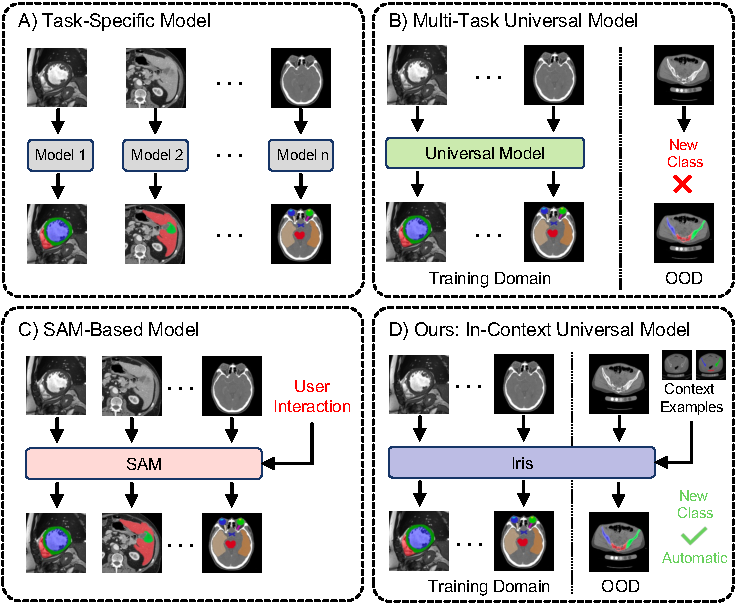
\includegraphics[width=0.47\textwidth]{./fig/paradigm_comparison.pdf}
\end{center}
\vspace{-1em}
\caption{Comparison of medical image segmentation approaches. A) Task-specific models require training separate models for each task, limiting their flexibility and scalability. B) Multi-task universal models can handle diverse tasks and imaging modalities, but fail on novel classes. C) SAM-based foundation models enable flexible segmentation through user interactions, but impractical for high-throughput automated processing. D) Our proposed Iris combines automatic processing with flexible adaptation via in-context learning, enabling both seen and unseen task segmentation without any manual interaction or retraining.}
\label{fig:fig1}
\vspace{-1em}
\end{figure}



% They can't as generalizable and adaptive as radiologist, challenges.
These task-specific methods show critical limitations compared to human experts' capabilities. First, existing models often perform poorly on out-of-distribution examples~\cite{zhou2022domain}—a common scenario in medical imaging where variations arise from different imaging centers, patient populations, and acquisition protocols. Second, traditional segmentation models, while achieving a high accuracy on their trained tasks, lack the adaptability to handle novel classes without extensive retraining or fine-tuning~\cite{zhang2023continual}. This dilemma fundamentally limits task-specific models' applicability in dynamic clinical settings and research environments, where new segmentation tasks continue to emerge over the course of real-world practice.



% Current solutions and limitations
Recent research has explored several directions to address these challenges (Figure \ref{fig:fig1}). Universal medical segmentation models~\cite{zhang2021dodnet,liu2023clip,ye2023uniseg,ulrich2023multitalent} attempt to leverage synergy among multiple tasks across diverse datasets to learn robust representations, yet struggling with unseen classes and requiring fine-tuning. Foundation models with interactive capabilities, such as SAM~\cite{kirillov2023segment} and its medical variants~\cite{zhang2024data,ma2024segment,cheng2023sam,wang2024sam}, offer flexibility via user prompts. But they require multiple interactions for optimal segmentation results, especially for complex 3D structures, and lack the efficiency for large-scale automated analysis. In addition, in-context learning (ICL) methods~\cite{butoi2023universeg,rakic2024tyche} show promise in automatically handling arbitrary new tasks through a few reference examples, but current methods exhibit suboptimal performance compared to task-specific models and suffer from computational inefficiencies, requiring expensive reference encoding during each inference step.






% Our solution
To address these fundamental challenges, we present Iris framework for universal medical image segmentation via in-context learning. At its core, Iris features a lightweight task encoding module that efficiently distills task-specific information from reference image-label pairs into compact task embeddings, which then guide the segmentation of target objects. Unlike existing ICL methods~\cite{butoi2023universeg,rakic2024tyche}, Iris decouples the task definition from query image inference, eliminating redundant context encoding while enabling flexible inference strategies, all coming with high computational efficiency. 

Our main contributions include:
\begin{itemize}
\item A novel in-context learning framework for 3D medical images, enabling a strong adaptation to arbitrary new segmentation tasks without model retraining or fine-tuning.
\item A lightweight task encoding module that captures task-specific information from reference examples, handling medical objects of varying sizes and shapes.
\item Multiple flexible inference strategies suitable for different practical scenarios, including one-shot inference, context ensemble, object-level context retrieval, and in-context tuning.
\item Comprehensive experiments on 19 datasets demonstrate Iris's superior performance across both in-distribution and challenging scenarios, particularly on held-out domains and novel anatomical structures. It extends to reveal the capability of automatically discovering meaningful anatomical relationships across datasets and modalities.
\end{itemize}



% Contribution
